\section{Materials and Methods}

\begin{figure}
\begin{center}
\begin{minipage}[t]{0.5\linewidth}

% \hspace*{\fill}%
\begin{minipage}[t]{\linewidth}
\centering
\vspace{0pt} % for alignment
\begin{minipage}{\textwidth}
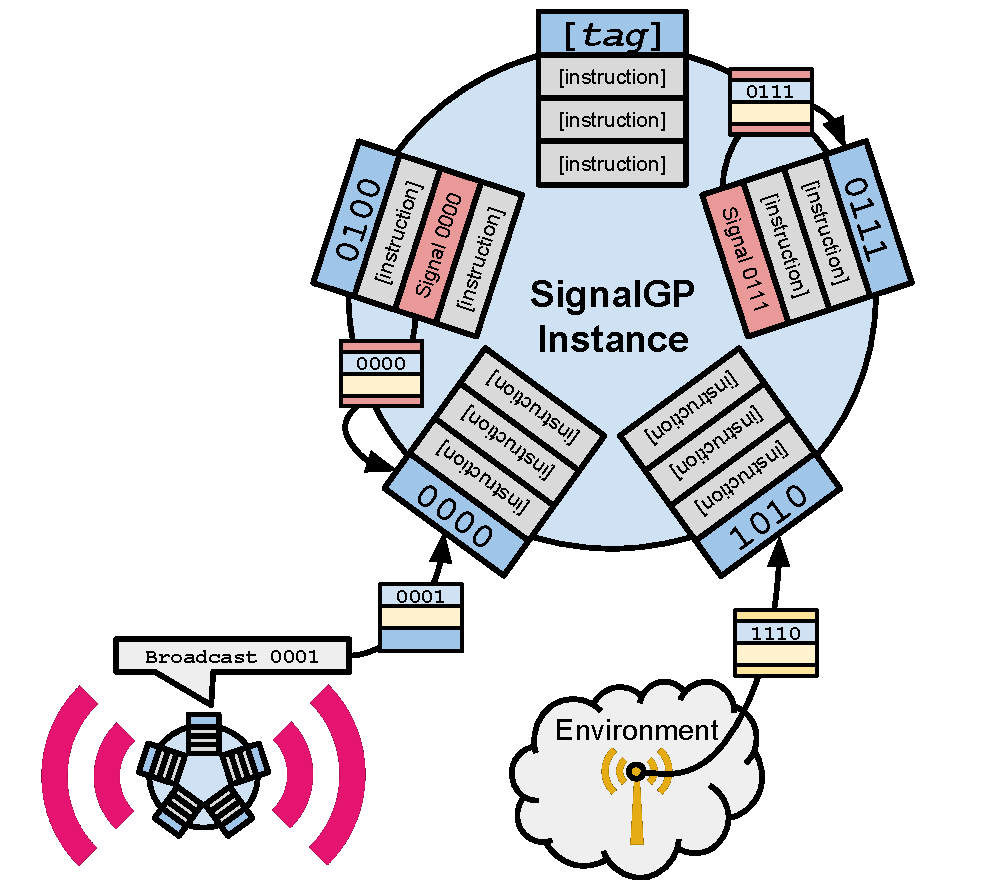
\includegraphics[width=\linewidth]{img/signalgp-cartoon}
{\textbf{(A)}
A cartoon overview of a single SignalGP instance.
SignalGP program modules execute pseudo-concurrently in response to tagged signals, which can originate internally, from the environment, or from other agents.
}
% \label{fig:signalgp-cartoon}
\end{minipage}
\end{minipage}%
% \hspace*{\fill}

% \hspace*{\fill}%
% \begin{minipage}[t]{\linewidth}
% \centering
% \vspace{0pt} % for alignment
% \begin{minipage}{\textwidth}
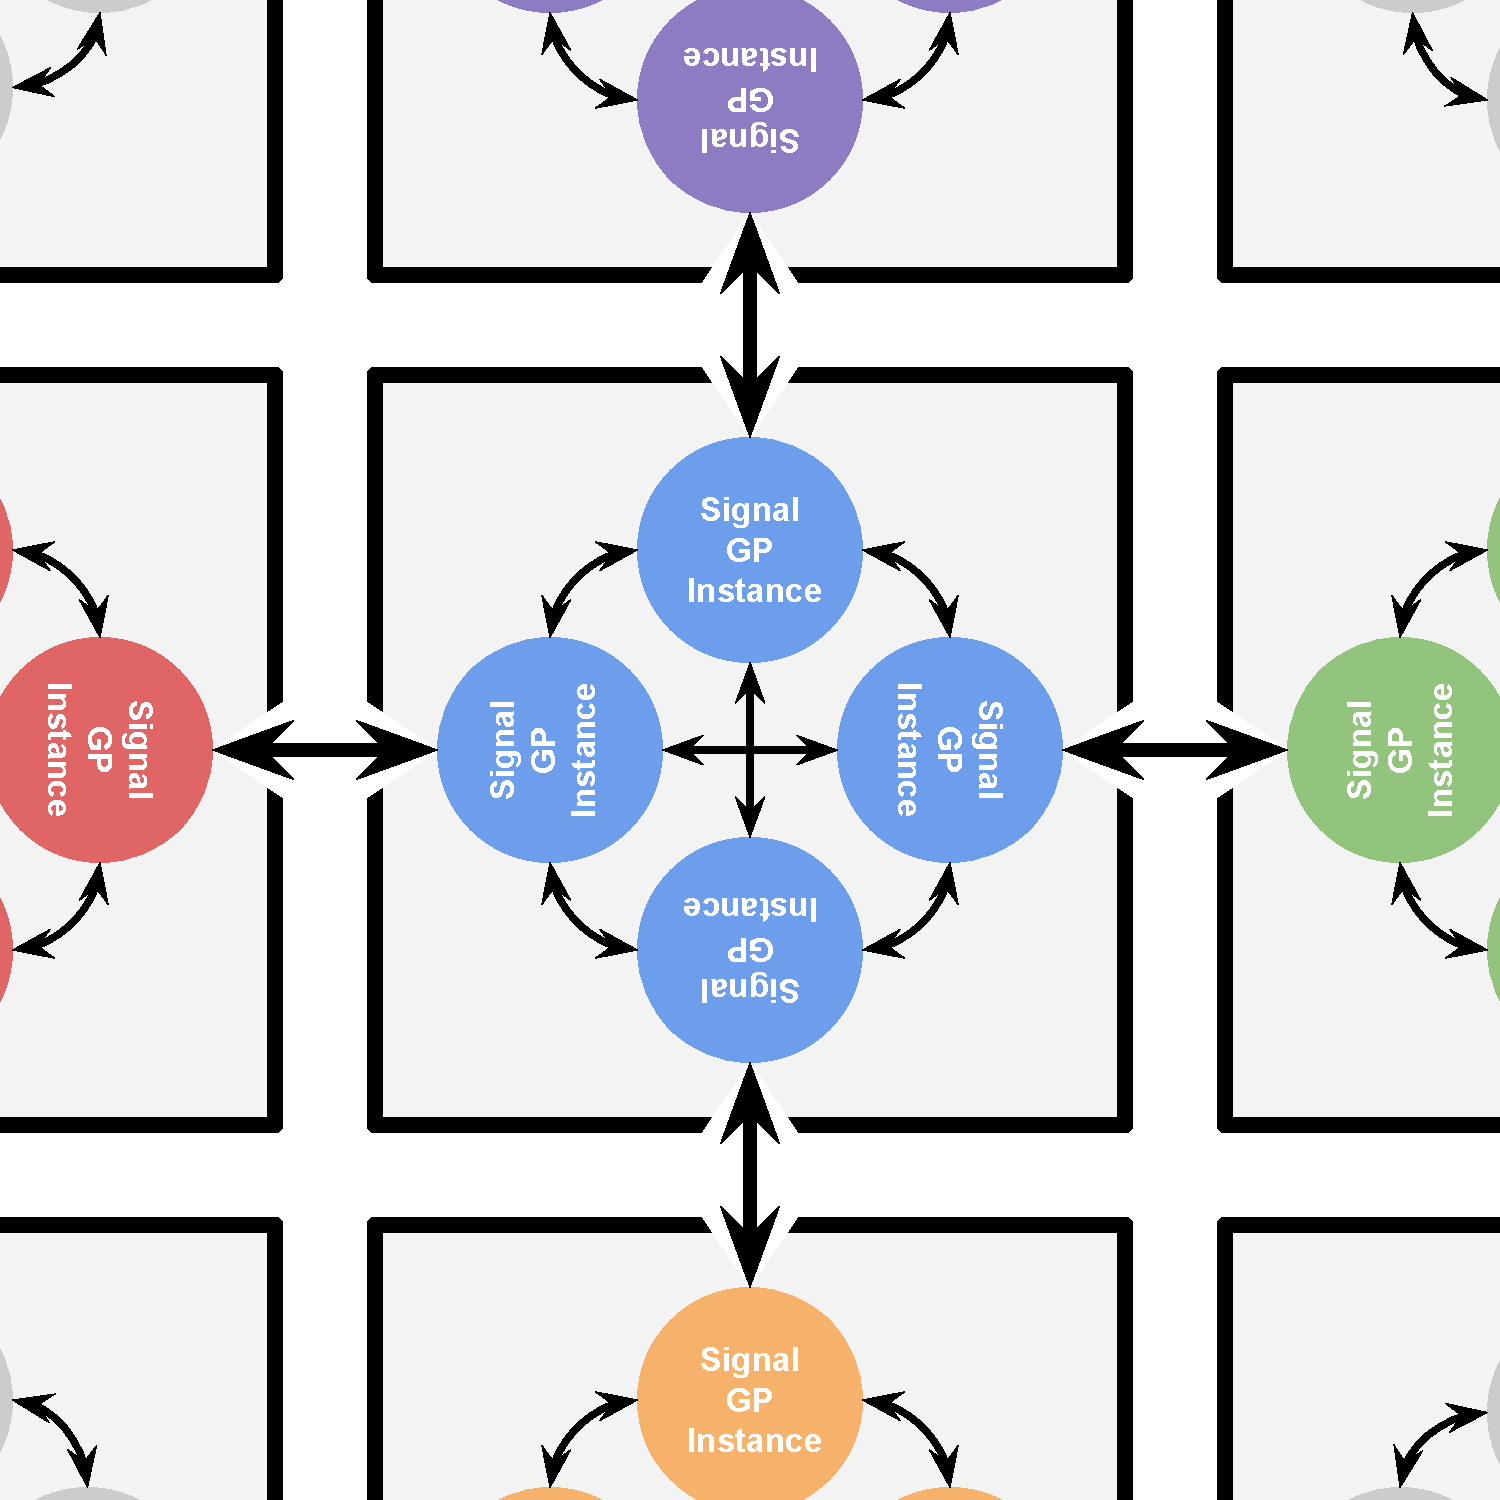
\includegraphics[width=0.8\linewidth]{img/dishtinygp-cartoon}\\
{\textbf{(B)}
A cartoon overview of how individual SignalGP instances are organized into DISHTINY cells.
% Each cell contains four independent SignalGP instances.
% The same genetic program is mirrored across all four SignalGP instances, but each instance executes independently.
Within each DISHTINY cell, each of four independent instances senses environmental state, receives intercellular messages, and determines cell behavior with respect to a single cardinal direction.
All four instances sense non-directional environmental cues and non-directional actions may be taken by any instance.
Instances within a cell communicate via intracellular messaging.
}
% \label{fig:dishtinygp-cartoon}
% \end{minipage}
% \end{minipage}%
% \hspace*{\fill}
\end{minipage}

\caption{
Schematic illustrations of how individual SignalGP instances function and how individual SignalGP instances are organized into DISHTINY cells.
Subfigure \textbf{(A)} provided courtesy Alexander Lalejini.
}
\label{fig:signalgp-dishtinygp}
\end{center}
\end{figure}


We performed simulations in which cells evolved open-ended behaviors to make decisions about resource sharing, reproductive timing, and apoptosis.
We will first describe the environment and hereditary grouping system cells evolved under and then describe the behavior-control system cells used.

\subsection{Cells and Hereditary Groups}

Cells occupy individual tiles on a toroidal grid.
Over discrete time steps (``updates''), cells can collect a resource.
Once sufficient resource has been accrued, cells may pay one unit of resource to place a daughter cell on an adjoining tile of the toroidal grid (i.e., reproduce), replacing any existing cell already there.
Collected resource decays at a rate of 0.1\% per update, incentivizing its quick use.

Cells accrue resource via a cooperative resource-collection process.
Cooperating in medium-sized groups (on the order of 100 cells) with a roughly circular layout accelerates per-cell resource collection rate.
Unicellular, too-small, too-large, or irregularly-shaped groups collect resource at a lesser per-cell rate.

Cells may grow a cooperative resource-collecting group through cell proliferation.
For this reason, we refer to these groups as ``hereditary groups.''
These hereditary groups develop through cell proliferation.
As cells reproduce, they can choose to adsorb daughter cells onto the parent's hereditary group or expel those offspring to found a new hereditary group.
These decisions affect the spatial layout of these hereditary groups and, in turn, affect individual cells' resource-collection rate.

To promote group turnover, we counteract the advantage of established hereditary groups with a simple aging scheme.
As hereditary groups age over elapsed updates and somatic generations, their constituent cells expressly lose the ability regenerate somatic tissue and then, soon after, to collect resource.

A complete description of the mechanisms behind these collective resource-collection and group aging mechanisms appears in Supplementary Sections \ref{sup:resource_collection_process} and \ref{sup:hereditary_group_life_cycle}.

Because new hereditary group IDs arise first in a single cell and grow disseminate exclusively among direct descendants of that progenitor cell, hereditary groups are reproductively bottlenecked.
This clonal (or ``staying together'') multicellular life history stands in contrast with an aggregative (or ``coming together'') life cycle where chimeric groups arise via fusion of potentially loosely-related lineages \citep{staps2019emergence}.
Such clonal development is known to strengthen between-organism selection effects \citep{grosberg2007evolution}.

In this work, we screen for fraternal transitions in individuality with respect to these hereditary groups by evaluating three characteristic traits of higher-level organisms: resource sharing, reproductive division of labor, and apoptosis.
We can further screen for the evolution of complex multicellularity by assessing cell-cell messaging, regulatory patterning, and functional differentiation between cells within hereditary groups \cite{knoll2011multiple}.

\subsection{Hierarchical Nesting of Hereditary Groups} \label{sec:hierarchical_nesting}

Successive fraternal transitions in natural history, for example to multicellularity and then to eusociality \citep{smith1997major}) underscores the constructive power of evolution to harness emergent structures as building blocks for further novelty.
To explore these dynamics, in some experimental conditions we incorporated a hierarchical extension to the hereditary grouping scheme described above.

Hierarchical levels are introduced into the system by providing a mechanism to groups of hereditary groups to form.
We accomplish this through two separate, but overlaid, instantiations of the hereditary grouping scheme.
We refer to each independent hereditary grouping system as a ``level.''
The hierarchical extension allows two levels of hereditary grouping, identified here as L0 and L1.
Without the hierarchical extension, only L0 is present.
\footnote{
We chose to number these levels using the computer science convention of zero-based indexing (as opposed to everyday practice of counting up from one) to maintain consistency with source code and data sets associated with this work.
}
We refer to the highest hereditary grouping level present in a simulation as the ``apex'' level.

Under the hierarchical extension, each cell contained a pair of separate hereditary group IDs --- the first for L0 and the second for L1.
During reproduction, daughter cells could either
\begin{enumerate}
\item inherit both L0 and L1 hereditary group ID,
\item inherit L0 hereditary group ID but not L1 hereditary group ID, or
\item inherit neither hereditary group ID.
\end{enumerate}
In order to enforce hierarchical nesting of hereditary group IDs, daughter cells could not inherit just the L1 hereditary group ID.

Hierarchically nested hereditary group IDs are analogous to a strict corporate organizational structure: all employees (i.e., cells) are members of one department (i.e., L0 hereditary group) and one corporation (i.e., L1 hereditary group) but no employee can be a member of two departments and no department can be a member of two corporations.
Useful as a concrete illustration of this scheme, Figure \ref{fig:morphology-wt} depicts hierarchically-nested hereditary groupings assumed by an evolved strain.

\subsection{Cell-Level Organisms}

Our experiments use cell-level digital organisms controlled by genetic programs subject to mutations and implicit selective pressures.

We employ the SignalGP event-(riven genetic programming representation.
As sketched in Figure \ref{fig:signalgp-cartoon}, this representation is specially designed to express function-like modules of code in response to internal signals or external stimuli.
This process can be considered somewhat akin to gene expression.
The event-driven framework facilitates the evolution of dynamic interactions between digital organisms and their environment (including other organisms) \citep{lalejini2018evolving}.

Special module components allow evolving programs to sense and interact with their environment, through mechanisms including resource sharing, hereditary group sensing, apoptosis, cell reproduction, and arbitrary cell-cell messaging.
Modules can also include general purpose computational elements like conditionals and loops, which allows cells to evolve sophisticated behaviors conditioned on current (and even previous) local conditions.

Previous work evolving digital organisms in grid-based problem domains has relied on a single computational agent that designates a direction to act in via an explicit cardinal ``facing'' \citep{goldsby2014evolutionary, goldsby2018serendipitous, grabowski2010early, biswas2014causes, lalejini2018evolving}.
Here, we introduce novel methodology to facilitate the evolution of directionally-symmetric phenotypes.
In this work, each cell instantiates four copies of the SignalGP hardware: one facing each cardinal direction.
These hardware instances all execute the same SignalGP program and may coordinate via internal signals, but are otherwise decoupled.
Figure \ref{fig:dishtinygp-cartoon} overviews the configuration of the four SignalGP instances that constitute a single cell.

Supplementary Sections \ref{sup:cell_level_organisms}, \ref{sup:standard_instruction_library}, \ref{sup:custom_instruction_library}, and \ref{sup:environmental_cue_library} provide full details of the digital evolution substrate underpinning this work.

\subsection{Surveyed Evolutionary Conditions}

To broaden our exploration of possible evolved multicellular behaviors in this system, we surveyed several evolutionary conditions.

In one manipulation, we explored the effect of structuring hereditary groups, such that parent cells can choose to keep offspring in their same sub-group, in just the same full group, or expel them entirely to start a new group.
Cells can independently mediate their behavior based on the level of the group with which they are interacting.

In a second manipulation, we explored the importance of explicitly selecting for medium-sized groups (as had been needed to maximize resource collection) by removing this incentive.
Instead, they system distributed resource at a uniform per-cell rate.

We combined these two manipulations to yield four surveyed conditions:
\begin{enumerate}
\item ``Flat-Even'': One hereditary group level (flat) with uniform resource inflow (even). In-browser simulation: \url{https://hopth.ru/i},
\item ``Flat-Wave'': One  hereditary group level (flat) with group-mediated resource collection (wave); In-browser simulation: \url{https://hopth.ru/j}),
\item ``Nested-Even'': Two hierarchically-nested hereditary group levels (nested) with uniform resource inflow (even). In-browser simulation: \url{https://hopth.ru/k},
\item ``Nested-Wave'': Two hierarchically-nested hereditary group levels (nested) with group-mediated resource collection (wave). In-browser simulation: \url{https://hopth.ru/l}.
\end{enumerate}

Supplementary Section \ref{sup:treatments} provides full details of surveyed evolutionary conditions.
